%% \listfiles
%\RequirePackage[2020-02-02]{latexrelease}
%\documentclass[iop]{emulateapj}
\documentclass[12pt]{article}
%\documentclass[preprint2,12pt]{emulateapj}
\usepackage{wrapfig}
\usepackage{float}
\usepackage{listings}

\usepackage{natbib}
\usepackage{graphicx}
\usepackage{epsfig}
\usepackage{amssymb,amsmath}
\usepackage{array}
\usepackage{threeparttable}

\usepackage{subcaption}

%\usepackage[strings]{underscore}
\usepackage{url}



%\singlespace

%definitions
\newcommand{\Msol}{${\rm M_{\sun}}$}
\newcommand{\boo}{\textit{Bo\"{o}tes III}}

%% Editing markup...
\usepackage{color}


%%%%%%%%%%%%%%%%%%%%%%%%%%%%%%%%%%%%%%%%%%%%%%%%%%%%%%%%%%%%%%%%%%%%%%%%%%%
% WARNING: This LaTeX block was generated automatically by authors.py
% Do not change by hand: your changes will be lost.

%%%%%%%%%%%%%%%%%%%%%%%%%%%%%%%%%%%%%%%%%%%%%%%%%%%%%%%%%%%%%%%%%%%%%%%%%%%


% --------------------- Ancillary information ---------------------
%\shortauthors{Anya Dovgal}
%\shorttitle{Bootes Stream Particle Generation}
%\slugcomment{Draft: \today}


\begin{document}


\title{CTA200H Project: Stream Particle Generation around Bo\"{o}tes III.}
 %% ---------
 
\author{Anya Dovgal}
%\altaffiltext{1}{SURP, University of Toronto, David A. Dunlap Department of Astronomy \& Astrophysics}
\maketitle 


\begin{abstract}
In this project, the kinematic properties of the dwarf spheroidal galaxy \boo are used to generate stream particles after it passes through the potential of the Milky Way. With the use of galpy \& streamtools \cite{Bovy_2015}, I simulated the orbit of \boo and its stream particles, under the assumption that tidal disruption started 5 years ago. I repeated the model under three different potentials. I also repeated the simulation using new data \cite{Pace_6D}, which gave different results. I found that the simulations produce a large amount of stream particles from \boo, particularly after the galaxy's last pass through the pericentre of its orbit.
After submission of this project, I plan to refine the scripts, as well as test how a change in other properties of \boo can affect the result \textit{(eg. I plan to run the simulation under different masses for \boo)}. I also plan to generate stream particles around other dwarf galaxies \textit{(eg. Antlia 2)}
\end{abstract}

%\keywords{cosmology: dynamics, galactic evolution, tidal streams}




\section{Introduction}
\label{sec:intro}

\boo is a dwarf spheroidal galaxy, 46kpc away \cite{Carlin_2009} which was originally labelled to be only a stellar overdensity. However, due to the large velocity dispersion and elongated extension of stellar candidates, there is evidence \cite{Carlin_2009} that it may be halfway between a bound dwarf galaxy, and an unbound tidal stream. In this project, my goal was simply to generate stream particles around dwarf galaxies. At first, I followed a demonstration on stream particle generation created by Professor Webb at UofT, but I have studied and expanded upon it for this project.

\subsection{Script Explanation}
Although I have 3 scripts, they all follow the same outline \& steps. First, it creates the orbit of the galaxy, given the 6D data and potential of choice. The orbits are also instantiated with the solar motion (U,V,W) = (-11.1, 24, 7.25). Next, the distribution functions for the leading stream particles and trailing stream particles are created, for a given disruption time of 5Gyrs. Then after re-shaping the output 6D arrays, they are instantiated into new Orbit objects, which tracks the 6D coordinates for each star during the disruption time. The script then plots a few different projections of the stream particles at current day, along with the orbit of \boo for the 3D projections \textit{(Note, the RA/Dec projection is not ideal yet)}.

Next, the script animates the orbits of the galaxy and stream particles over the 5Gyrs since disruption. This animation includes the position of the Milky Way for clarity.

Lastly, the script repeats the first stream particle generation but with the inclusion of the LMC potential. This is done by first generating the LMC using data from SIMBAD and calculating its potential, then recalculating the stream distribution function, making sure to specify the potential used to calculate the tidal radius to be the MW potential w/out inclusion of the LMC. Then the script creates orbit objects for the new stream particles and plots the projection of stream particles at current day, compared to the particles calculated without the LMC.

\section{Data}
\label{sec:data}
Modelling of the stream particles is done using data extracted from the SIMBAD database, using \textit{galpy from-name}. I also took the mass estimate to be 
\begin{equation}
M(<r_{1/2}) \approx 1.82x10^7 \frac{R_{eff}}{100pc}
\label{eq:1}
\end{equation}
from \cite{Carlin_2009}, and then used the radius estimate of 0.5kpc \cite{Correnti_2009}

I also ran the simulation with data from Dr. Andrew Pace \cite{Pace_6D}. I used the same mass estimate as \ref{eq:1}.


\section{Calculations}
I had enough time to simulate 4 scenarios. I simulated one for data from SIMBAD under galpy's MWPotential2014, and then I simulated 3 with Dr. Pace's data, under MWPotential2014, MWPotential2014 with the mass doubled (so that I could compare with \cite{Carlin_2018}), and lastly with the deprecated MWPotential. For each simulation, I produced 2D and 3D plots for RA/Dec and cartesian projections of the streams, as well as a 3D video simulating the dynamics over the past 5Gyrs. I also compared the stream shape produced by the simulation with the inclusion of the LMC in the potential.

\begin{figure}[H]
\begin{subfigure}{.45\textwidth}
  \centering
  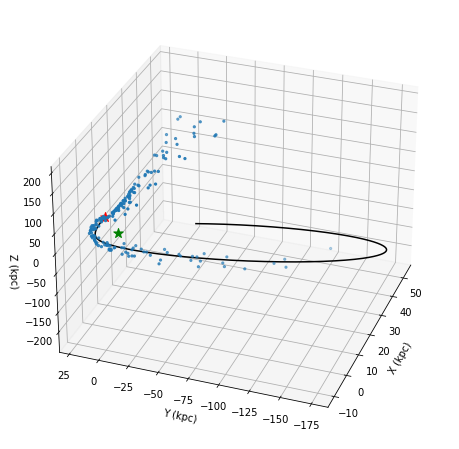
\includegraphics[width=\linewidth]{MWPot2014_orbit_fn.png}
  \caption{SIMBAD data under MWPotential2014}
  \label{fig:1.1}
\end{subfigure}
\begin{subfigure}{.45\textwidth}
  \centering
  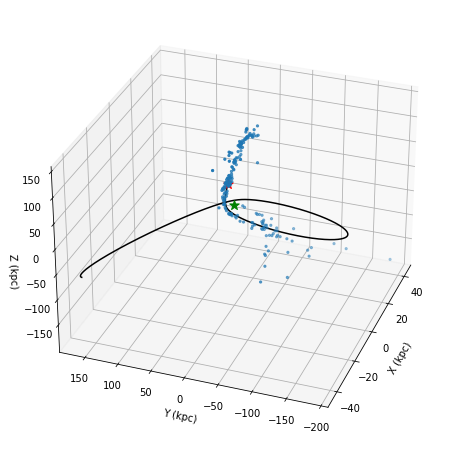
\includegraphics[width=\linewidth]{MWPot2014_orbit_AP6D.png}
  \caption{Dr. Pace data under MWPotential2014}
  \label{fig:1.2}
\end{subfigure}
\begin{subfigure}{.45\textwidth}
  \centering
  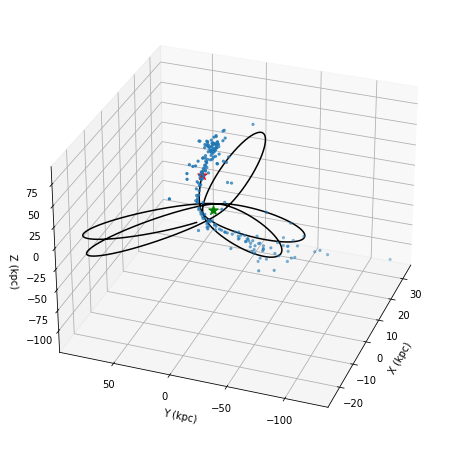
\includegraphics[width=\linewidth]{MWPot2014x2_orbit_AP6D.png}
  \caption{Dr. pace data under MWPotential2014 with MW mass doubled}
  \label{fig:1.3}
\end{subfigure}
\begin{subfigure}{.45\textwidth}
  \centering
  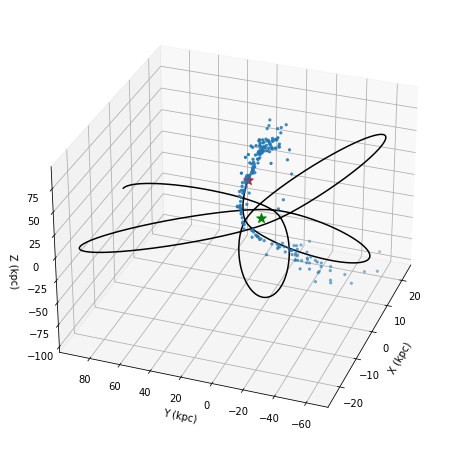
\includegraphics[width=\linewidth]{MWPot_orbit_AP6D.png}
  \caption{Dr. Pace data under MWPotential}
  \label{fig:1.4}
\end{subfigure}
\caption{Cartesian projections of orbit (black) and stream (blue) over last 5Gyrs}
\label{fig:1}
\end{figure}

\pagebreak

\section{Results}
I found that \boo generates a large amount of stream particles from the simulation, especially after its most recent pass through its orbit's pericentre, as seen very noticeably in \ref{fig:1.1} and \ref{fig:1.2}. Some of the stream simulations had an interesting shape/orientation, which I would like to study further to see if it is a fluke, or if it physically makes sense.
I have 4 videos in my repository starting with 'XYZ', with a suffix of 'AP6D' referring to Dr. Pace's data being used for the simulation, and 'fn' referring to the SIMBAD data.
Upon submission of this project, I would like to properly compare my results to those of \cite{Carlin_2018}.

\begin{figure}[H]
\begin{subfigure}{.45\textwidth}
  \centering
  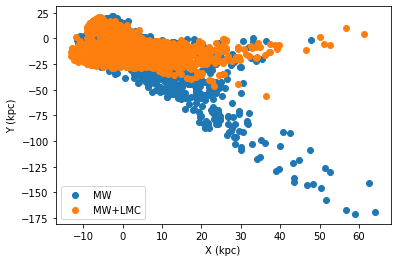
\includegraphics[width=\linewidth]{MWPot2014_wLMC_fn.png}
  \caption{SIMBAD data under MWPotential2014}
  \label{fig:2.1}
\end{subfigure}
\begin{subfigure}{.45\textwidth}
  \centering
  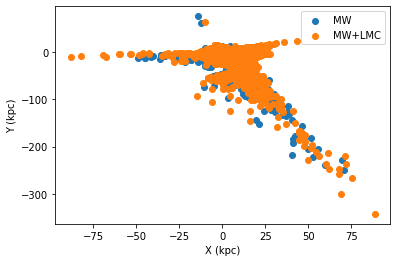
\includegraphics[width=\linewidth]{MWPot2014_wLMC_AP6D.png}
  \caption{Dr. Pace data under MWPotential2014}
  \label{fig:2.2}
\end{subfigure}

\caption{Cartesian projections of stream particles with and without including the LMC potential}
\label{fig:2}
\end{figure}


%\subsection{Subsection 1}
%\label{sec:cmb_data}
%This is a sub-section.
%Here is an equation:
%\begin{equation}
%E = mc^2
%\label{eq:relativity}
%\end{equation}
%Here is an example of math-mode in the main text: $a^2 + b^2 = c^2$.  Here is a reference, to Fig.~\ref{fig:figureOfSpectrum}.  The data section is section \ref{sec:data}.
%
%
%\begin{figure}
%\includegraphics[width=1.05\columnwidth]{plotAllPatches_Polonly.pdf}
%\caption{Here is how we insert a pdf figure.  This one is stolen from van Engelen+ 2014.\vspace{3mm}}
%\label{fig:figureOfSpectrum}
%\end{figure}
%
%
%
%\begin{table}
%\begin{center}
%\begin{threeparttable}
%\caption{A table.}
%\begin{tabular}{|l|c|c|}
%\hline 
%Col 1 & Col 2 & Col 3 \\
% \hline  
%Val 1 & Val 2 & Val 3 \\
%Val 1 & Val 2 & Val 3 \\
%\hline
%\end{tabular} 
%\vskip 2mm
%\begin{tablenotes} \item  
%\begin{center}
%\begin{flushleft}
%Description of table.
%\end{flushleft}
%\end{center}
%\end{tablenotes}
%\label{tab:vitalStats_kappa}
%\end{threeparttable}
%\end{center}
%\end{table}
%

%\acknowledgments

%\bibliographystyle{act}
%\bibliographystyle{apj}

%\bibliography{lenscib_refs.bib,apj-jour}

\pagebreak

%\begin{thebibliography}
\bibliography{biblio}
\bibliographystyle{unsrt}
%\end{thebibliography}

\end{document}